\documentclass[tikz,border=5pt]{standalone}
\usepackage[UTF8]{ctex}\usepackage{amsmath,amssymb}
\usetikzlibrary{arrows.meta,calc}
\definecolor{ink}{HTML}{243447}\definecolor{blue}{HTML}{2765A2}
\definecolor{green}{HTML}{3F7D5B}\definecolor{red}{HTML}{B74739}
\tikzset{body/.style={draw=ink,thick},vec/.style={draw=blue,thick,-{Latex}},guide/.style={gray!65,dashed},line cap=round,line join=round}
\newcommand{\edge}[3]{\draw[body](#1)--(#2)node[midway,fill=white,inner sep=2pt]{$#3$};}
\begin{document}
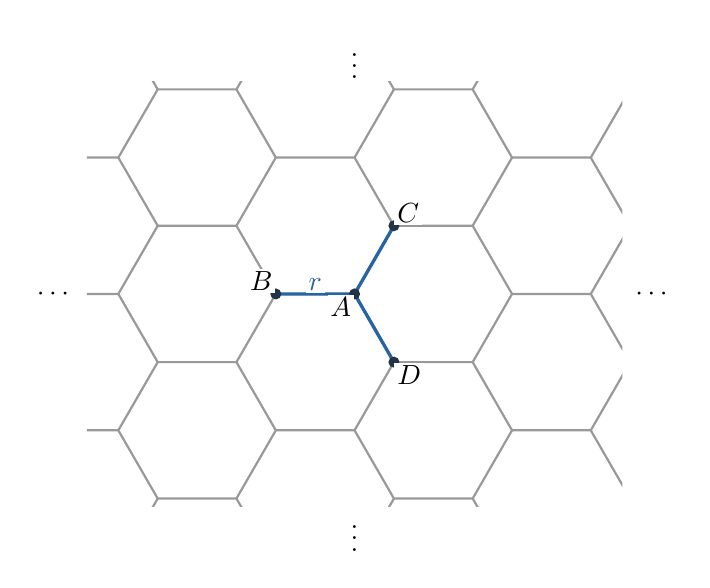
\begin{tikzpicture}
  \begin{scope}\clip(-3.4,-2.7)rectangle(3.4,2.7);
    \foreach\i in{-4,...,4}{\foreach\j in{-4,...,4}{
      \pgfmathsetmacro{\xx}{1.5*(\i+\j)}\pgfmathsetmacro{\yy}{.8660254*(\i-\j)}
      \draw[gray!80,thick](\xx,\yy)--({\xx-1},\yy)
      (\xx,\yy)--({\xx+.5},{\yy+.8660254})
      (\xx,\yy)--({\xx+.5},{\yy-.8660254});
    }}
  \end{scope}
  \coordinate(A)at(0,0);\coordinate(B)at(-1,0);\coordinate(C)at(.5,.8660254);\coordinate(D)at(.5,-.8660254);
  \draw[blue,very thick](B)--(A)--(C)(A)--(D);
  \foreach\p in{A,B,C,D}{\fill[ink](\p)circle(2pt);}
  \node[below left,fill=white,inner sep=1pt]at(A){$A$};
  \node[above left,fill=white,inner sep=1pt]at(B){$B$};
  \node[above right,fill=white,inner sep=1pt]at(C){$C$};
  \node[below right,fill=white,inner sep=1pt]at(D){$D$};
  \node[blue,above,fill=white,inner sep=1pt]at(-.5,0){$r$};
  \node at(-3.8,0){$\cdots$};\node at(3.8,0){$\cdots$};
  \node at(0,3){$\vdots$};\node at(0,-3){$\vdots$};
\end{tikzpicture}
\begin{tikzpicture}
  \foreach\k/\title in{0/{B注入，远处取出},1/{远处注入，C取出},2/{B注入，C取出}}{
    \begin{scope}[xshift=\k*4.4cm]
      \coordinate(A)at(0,0);\coordinate(B)at(-1.5,0);\coordinate(C)at(.75,1.3);\coordinate(D)at(.75,-1.3);
      \draw[gray!60](B)--(A)--(C)(A)--(D);
      \node[below left]at(A){$A$};\node[left]at(B){$B$};\node[above]at(C){$C$};\node[below]at(D){$D$};
      \ifnum\k=0
        \draw[vec](B)--(A)node[midway,above]{$I/3$};
        \draw[vec](A)--(C)node[midway,left]{$I/6$};
        \draw[vec](A)--(D)node[midway,left]{$I/6$};
      \fi
      \ifnum\k=1
        \draw[vec](B)--(A)node[midway,above]{$I/6$};
        \draw[vec](A)--(C)node[midway,left]{$I/3$};
        \draw[vec](D)--(A)node[midway,left]{$I/6$};
      \fi
      \ifnum\k=2
        \draw[vec](B)--(A)node[midway,above]{$I/2$};
        \draw[vec](A)--(C)node[midway,left]{$I/2$};
        \node[right]at(.45,-.75){$0$};
      \fi
      \node[align=center]at(-.2,-2){\title};
    \end{scope}
  }
\end{tikzpicture}
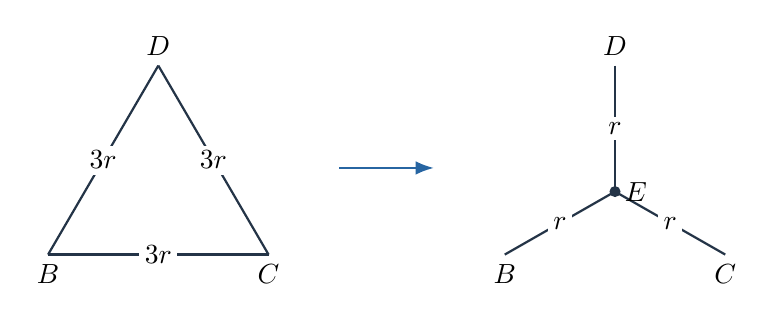
\begin{tikzpicture}
  \coordinate(B)at(-1.4,-1);\coordinate(C)at(1.4,-1);\coordinate(D)at(0,1.4);
  \edge{B}{C}{3r}\edge{B}{D}{3r}\edge{C}{D}{3r}
  \node[below]at(B){$B$};\node[below]at(C){$C$};\node[above]at(D){$D$};
  \draw[vec](2.3,.1)--(3.5,.1);
  \begin{scope}[xshift=5.8cm]
    \coordinate(B)at(-1.4,-1);\coordinate(C)at(1.4,-1);\coordinate(D)at(0,1.4);\coordinate(E)at(0,-.2);
    \edge{B}{E}{r}\edge{C}{E}{r}\edge{D}{E}{r}
    \node[below]at(B){$B$};\node[below]at(C){$C$};\node[above]at(D){$D$};\node[right]at(E){$E$};
    \fill[ink](E)circle(2pt);
  \end{scope}
\end{tikzpicture}
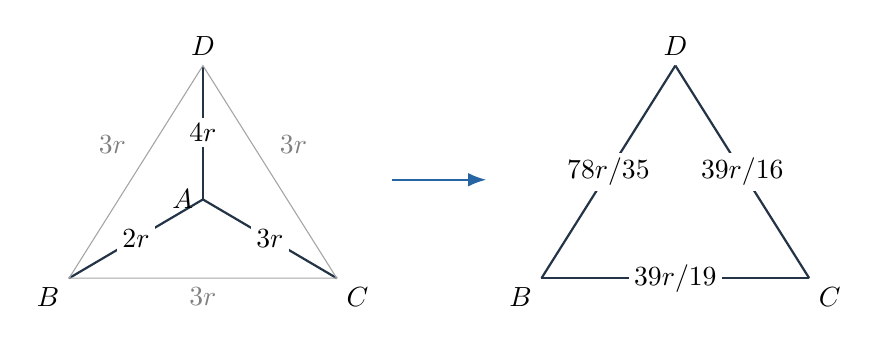
\begin{tikzpicture}
  \coordinate(B)at(-1.7,-1);\coordinate(C)at(1.7,-1);\coordinate(D)at(0,1.7);\coordinate(A)at(0,0);
  \edge{A}{B}{2r}\edge{A}{C}{3r}\edge{A}{D}{4r}
  \draw[gray!70](B)--(C)--(D)--cycle;
  \node[gray]at(-1.15,.7){$3r$};\node[gray]at(1.15,.7){$3r$};\node[gray,below]at(0,-1){$3r$};
  \node[left]at(A){$A$};\node[below left]at(B){$B$};\node[below right]at(C){$C$};\node[above]at(D){$D$};
  \draw[vec](2.4,.25)--(3.6,.25);
  \begin{scope}[xshift=6cm]
    \coordinate(B)at(-1.7,-1);\coordinate(C)at(1.7,-1);\coordinate(D)at(0,1.7);
    \edge{B}{C}{39r/19}\edge{B}{D}{78r/35}\edge{C}{D}{39r/16}
    \node[below left]at(B){$B$};\node[below right]at(C){$C$};\node[above]at(D){$D$};
  \end{scope}
\end{tikzpicture}
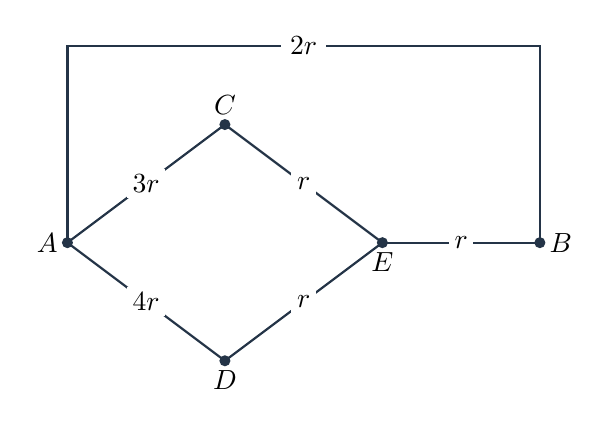
\begin{tikzpicture}
  \coordinate(A)at(0,0);\coordinate(B)at(6,0);\coordinate(E)at(4,0);
  \coordinate(C)at(2,1.5);\coordinate(D)at(2,-1.5);
  \draw[body](A)--(0,2.5)--(6,2.5)--(B);\node[fill=white]at(3,2.5){$2r$};
  \edge{A}{C}{3r}\edge{C}{E}{r}\edge{A}{D}{4r}\edge{D}{E}{r}\edge{E}{B}{r}
  \foreach\p in{A,B,C,D,E}{\fill[ink](\p)circle(2pt);}
  \node[left]at(A){$A$};\node[right]at(B){$B$};\node[above]at(C){$C$};\node[below]at(D){$D$};\node[below]at(E){$E$};
\end{tikzpicture}
\end{document}
